\section[Continuous integration]{Continuous integration}
\begin{frame}
	\frametitle{Continuous integration}
	\begin{columns}
		\begin{column}{0.4\textwidth}
			\begin{itemize}[<+->]
				\item Did anyone notice?
				\item For GitHub travis is a good alternative
				\item Jenkins also works with GitHub and supports MATLAB unlike travis
				\item BitBucket has bamboo, but may cost money
			\end{itemize}
		\end{column}
		\begin{column}{0.6\textwidth}
			\begin{figure}
				\centering
				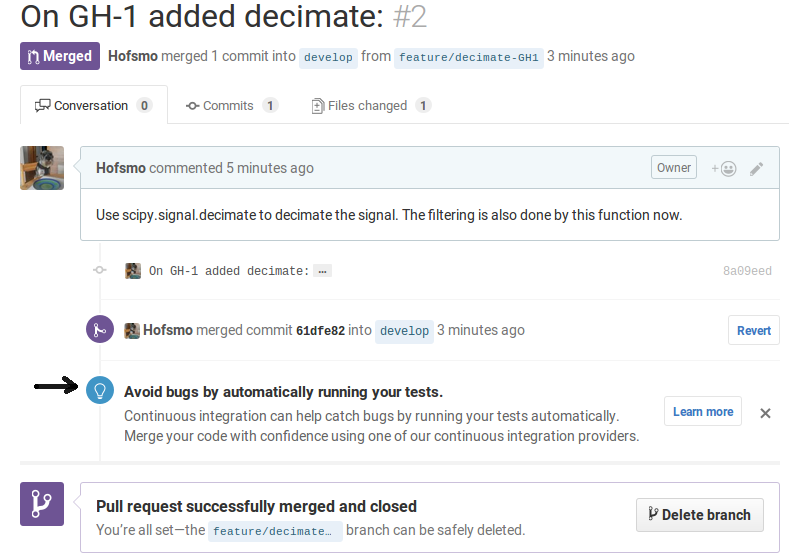
\includegraphics[width=\textwidth]{./pictures/cont.png}
			\end{figure}
		\end{column}
	\end{columns}
\end{frame}
\begin{frame}
	\frametitle{Travis}
	\begin{columns}
		\begin{column}{0.4\textwidth}
			\begin{itemize}[<+->]
				\item Travis is free for open repositories
				\item It is controlled through a configuration file named .travis.yml
				\item Does not support MATLAB
			\end{itemize}
		\end{column}
		\begin{column}{0.6\textwidth}
			\begin{figure}
				\centering
				
\includegraphics[width=\textwidth]{./pictures/Travis.eps}
			\end{figure}
		\end{column}
	\end{columns}
\end{frame}
